%------------------------------------------------------------------------------
\section{Methods}


%------------------------------------------------------------------------------
\FloatBarrier
\subsection{Artifact elimination}
\label{sec:ma}

Looking at rasters generated to include all the trials across all the sessions, an anomaly was apparent.
For several of the channels in the data from each of the brain regions of each of the animals, some sessions have spikes which align at the same time relative to the stimulus onset.
The temporal alignment is very precise, indicating the effect not part of the animal's brain activity but instead due to an external source influencing the detected signal in the recordings.
Furthermore, the ``lines'' occurred at regularly spaced intervals, with a period very nearly equal to the refresh rate of the monitor.
The spikes across multiple trials line up like this because the experimental equipment will only begin presenting a stimulus when the first pixel on the monitor is being updated, and we of course normalise for the stimulus presentation time across multiple trials.
% INCLUDE RASTER EXAMPLE

An empirical estimate of the artifact periodicity was found by choosing an arbitrary channel which strongly expresses the artifact and measuring by eye the duration of the completed artifact cycles within \SI{530}{ms} (44 for \ac{M1}, 39 for \ac{M2}).
Since the artifact is tightly localised in time, this could be done with relatively high accuracy.
For \ac{M1}, the period was estimated to be \SI{85.023(1)}{Hz}, whilst for \ac{M2} it was \SI{75.023(1)}{Hz}.
The discrepancies from the programmed monitor refresh rates of \SI{85}{Hz} and \SI{75}{Hz} respectively can be put down to the specific electronic circuitry used, perhaps issuing the command to the monitor.
The discrepancy is small enough to be of little consequence, except we will need \SI{5}{sf} of accuracy rather than \SI{2}{sf} in the following treatment of the artifact.
Why it should be out by exactly \SI{0.023}{Hz} for both animals remains unclear, since this corresponds to the refresh cycle running \SI{0.0031}{ms} fast for \ac{M1} and \SI{0.0042}{ms} fast for \ac{M2}.
An even bigger mystery is how the artifact has made its way into the recordings.
Although it remains possible that the cause is some other piece of equipment also locked to the same refresh cycle, in the following we will refer to this artifact as the ``monitor artifact''.
When a collection of data points exhibits the monitor artifact, we refer to the data as ``contaminated''.

From the rasters, it seemed as if three-quarters of the channels in \ac{M1} \ac{V4} were contaminated for at least one session; over two-thirds of the channels for \ac{M1} \ac{V1} and \ac{M2} \ac{V4} were contaminated for at least one session; and around a third of the channels for \ac{M2} \ac{V4} were contaminated for at least one session.
The contaminated channels include both high-quality channels with a lot of detected spikes, and low-quality channels with fewer detected spikes.
For some of the lowest quality channels and sessions, the artificial spikes were clearly more numerous than the genuine ones.
It was considered paramount that the effects of the artifact be corrected for.

To clean up the contamination, a more rigorous method of evaluating the problem was required.
For the collection of spike times from a single channel across multiple trials during a single session, we perform the following steps:
\begin{enumerate}
\item Consider the set of all spike times where the visual stimulus has been the same for at least the last \SI{150}{ms}.
\item From each spike time, $t$, subtract time of nearest stimulus onset/offset, $T_{\text{onset}}$.
      (Both onset and offset are synchronised with the monitor cycle, and the nearest one offers greatest accuracy.)
$$
t \leftarrow t - T_{\text{onset}}
$$
\item Take the modulo of the spike times with respect to the monitor period, $\tau_m$ (\SI{11.7616}{ms} for \ac{M1}, \SI{13.3292}{ms} for \ac{M2}).
$$
t \leftarrow t \bmod \tau_m
$$
\item Take a histogram of the spike times over bins with the width of the reciprocal of the sampling frequency of the spikes (sampling frequency \SI{32556.000}{Hz}; bin width \SI{0.030716}{ms}).
\end{enumerate}
Conceptually, this is equivalent to stacking all the ``lines'' in the raster on top of each other and seeing how thick the resulting line is.
When the visual stimulus has remained unchanged for at least \SI{150}{ms}, the neurons in \ac{V1} and \ac{V4} settle down to a steady firing rate, so we expect there to be about the same number of spikes in each of these bins.
However, as the monitor artifact increases the number of spikes at set intervals after the monitor refresh commences, there will be an increase in the number of spikes in these bins when the monitor artifact is manifest in the data.

% figs/info/monitor_hist_blanco_v4_ch4_s336_20120817T085037.eps
% figs/info/monitor_hist_jack_v1_ch9_s51_20120817T084845.eps
% figs/info/monitor_hist_jack_v1_ch9_s56_20120817T084855.eps
% figs/info/monitor_hist_jack_v4_ch41_s31_20120817T085111.eps
%%\begin{figure}[htbp]
%%    \begin{subfigure}[b]{0.5\linewidth}
%%        \centering
%%        \caption{}
%%        \label{fig:mahist-b4}
%%        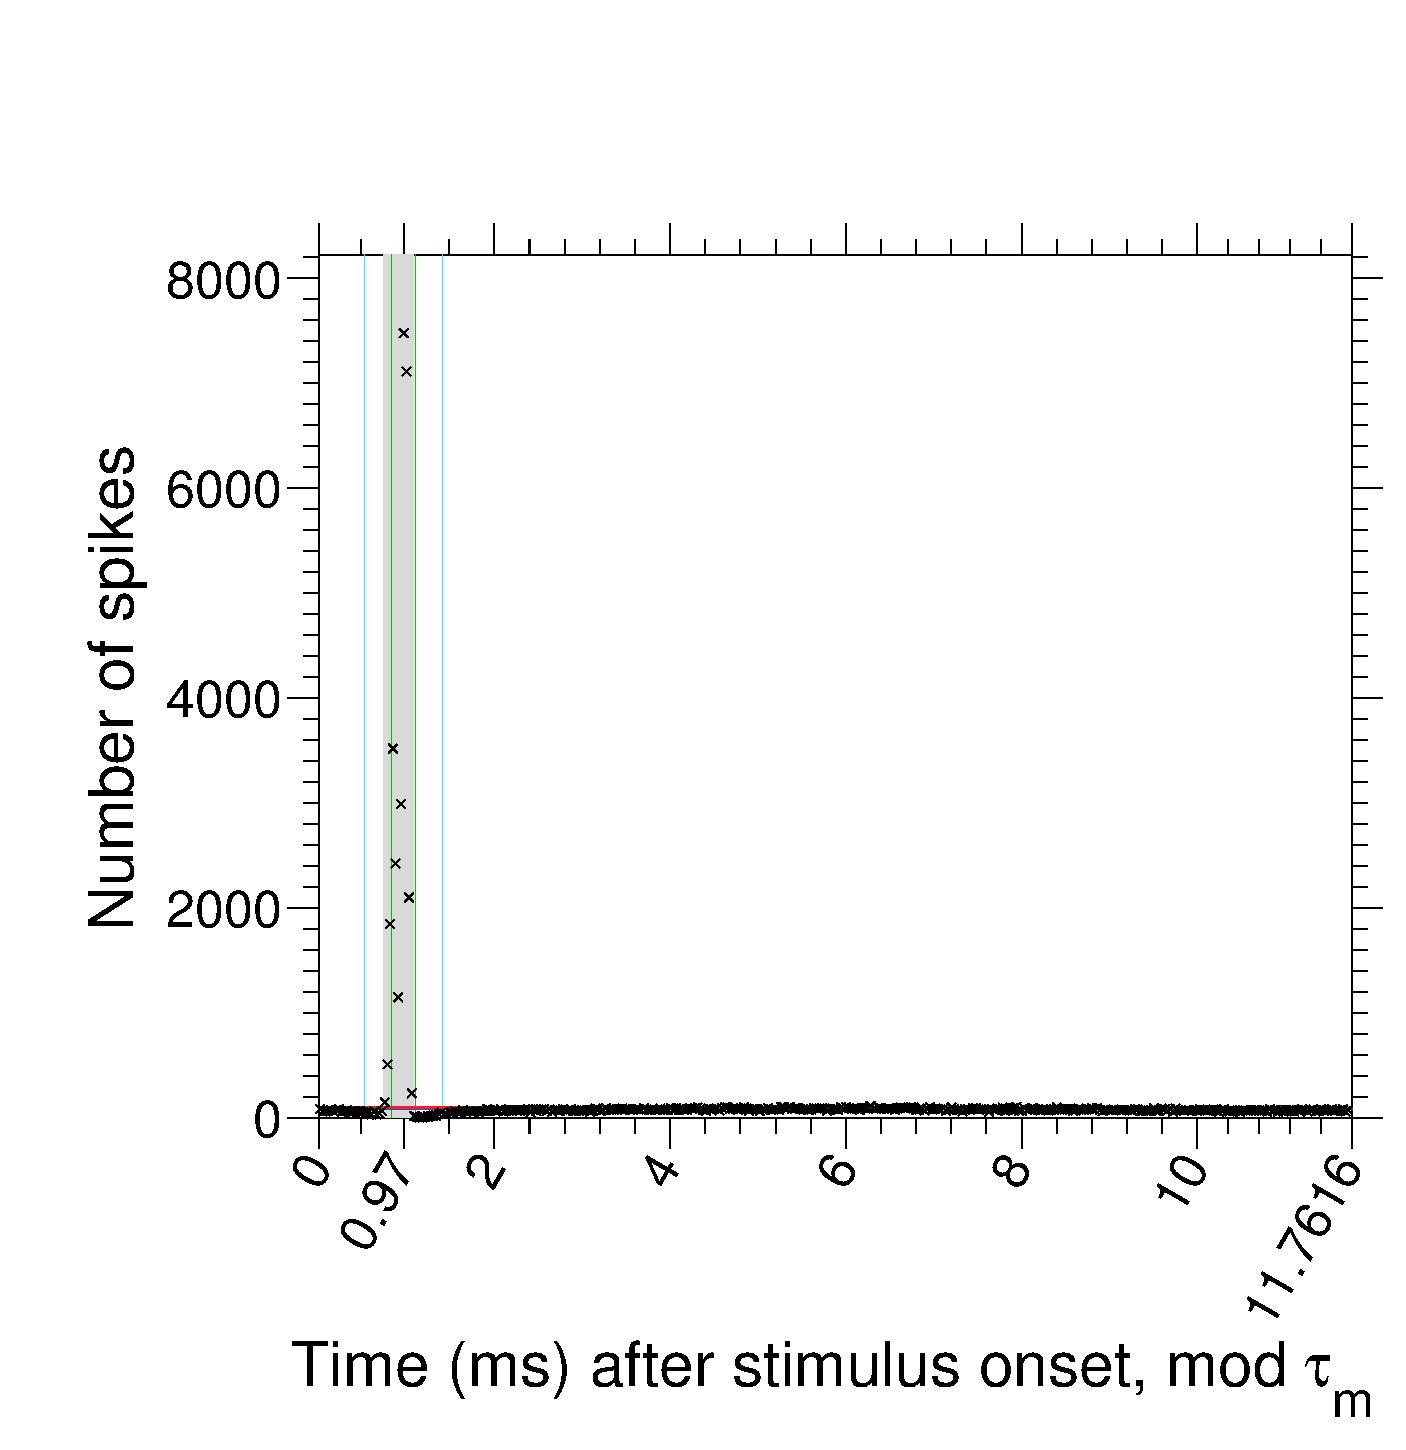
\includegraphics[width=\linewidth]{%
%%figs/info/monitor_hist_blanco_v4_ch4_s336_20120817T085037.eps}
%%    \end{subfigure}
%%    ~~
%%    \begin{subfigure}[b]{0.5\linewidth}
%%        \centering
%%        \caption{}
%%        \label{fig:mahist-j4}
%%        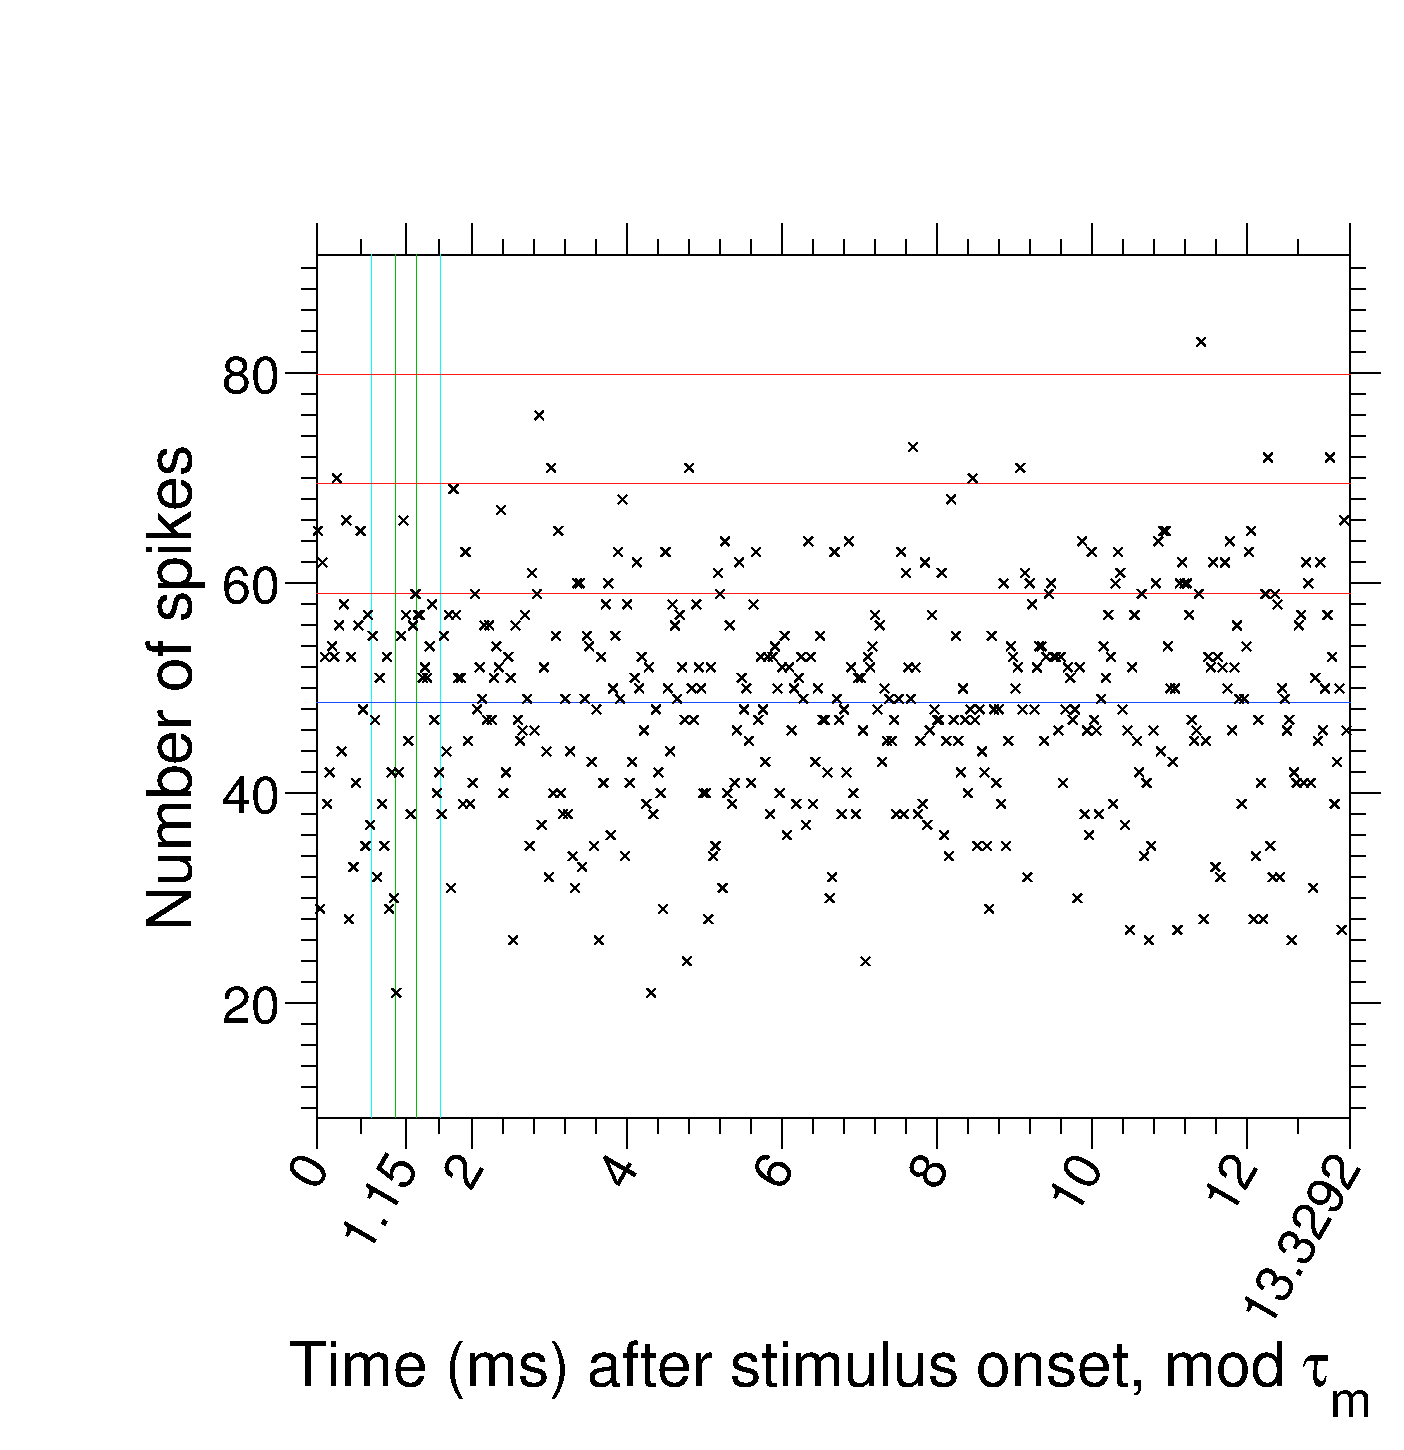
\includegraphics[width=\linewidth]{%
%%figs/info/monitor_hist_jack_v4_ch41_s31_20120817T085111.eps}
%%    \end{subfigure}
%%    \\
%%    \begin{subfigure}[b]{0.5\linewidth}
%%        \centering
%%        \caption{}
%%        \label{fig:mahist-j1s51}
%%        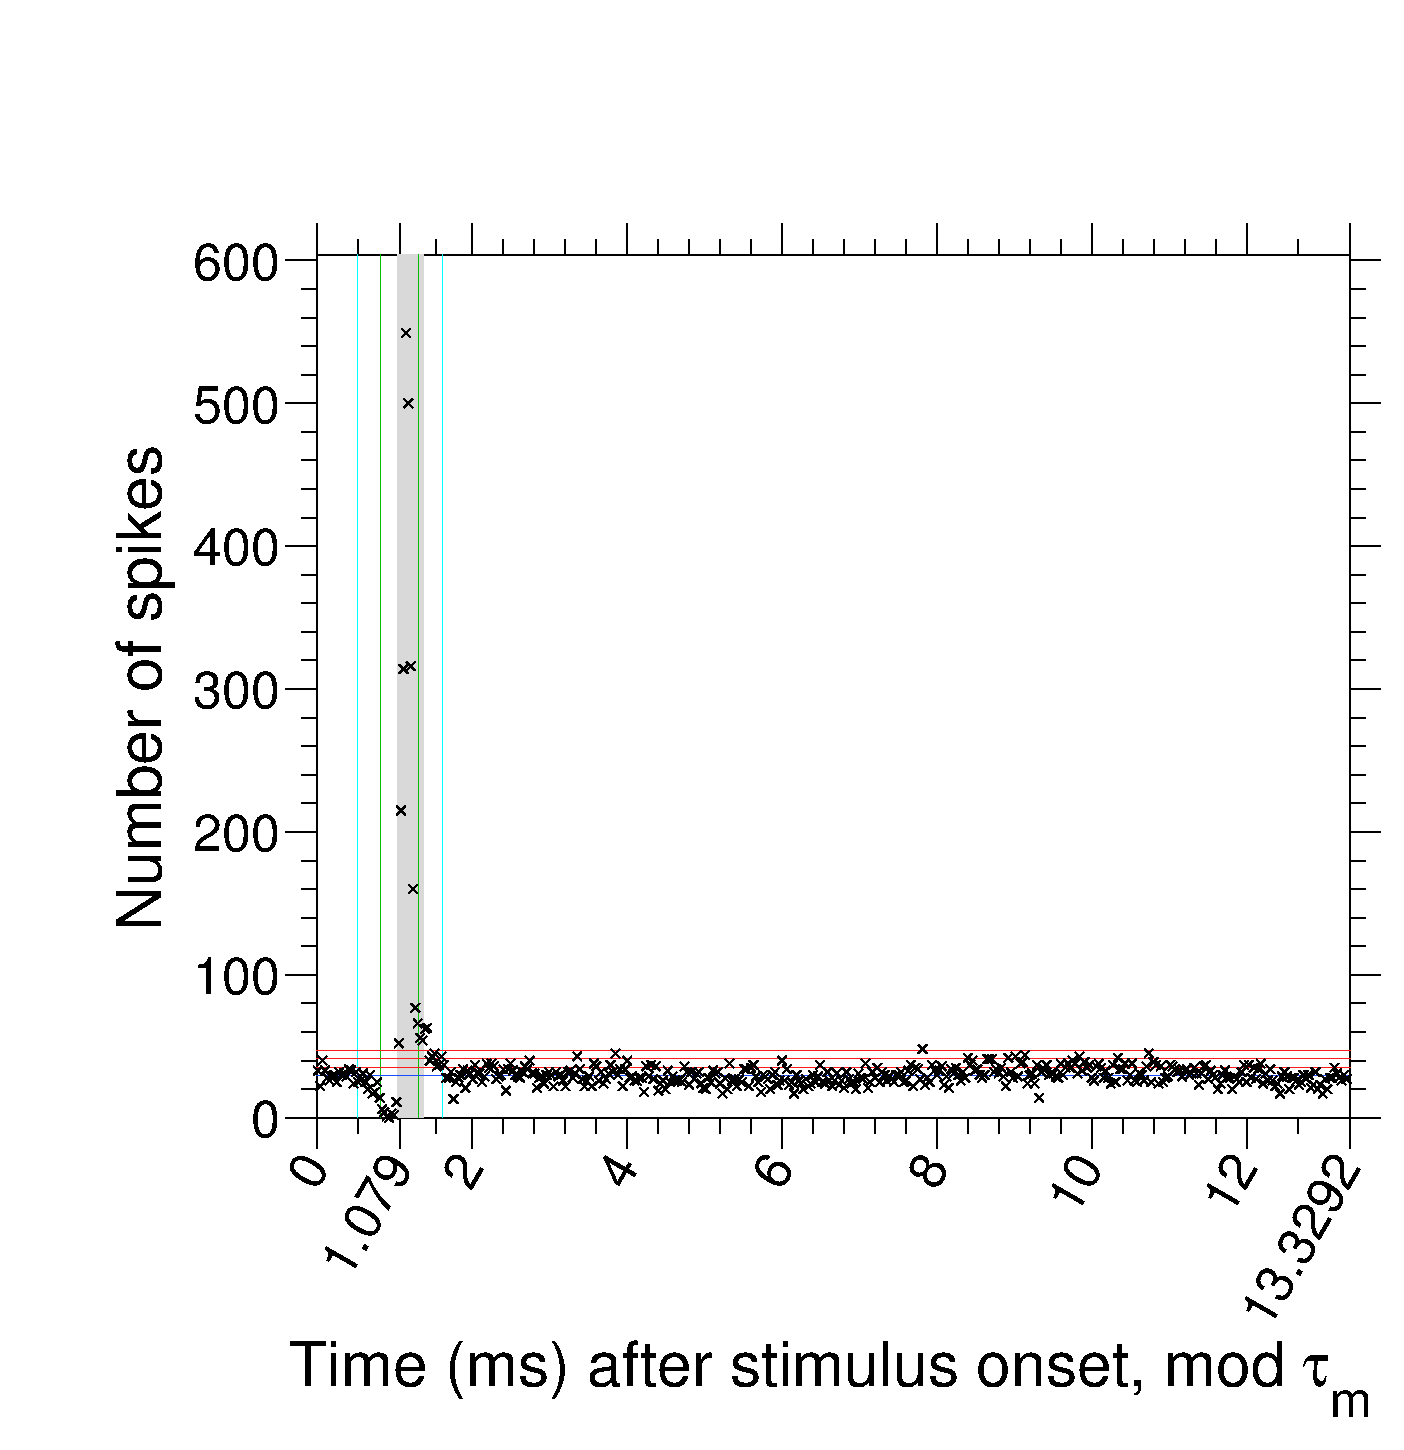
\includegraphics[width=\linewidth]{%
%%figs/info/monitor_hist_jack_v1_ch9_s51_20120817T084845.eps}
%%    \end{subfigure}
%%    ~~
%%    \begin{subfigure}[b]{0.5\linewidth}
%%        \centering
%%        \caption{}
%%        \label{fig:mahist-j1s56}
%%        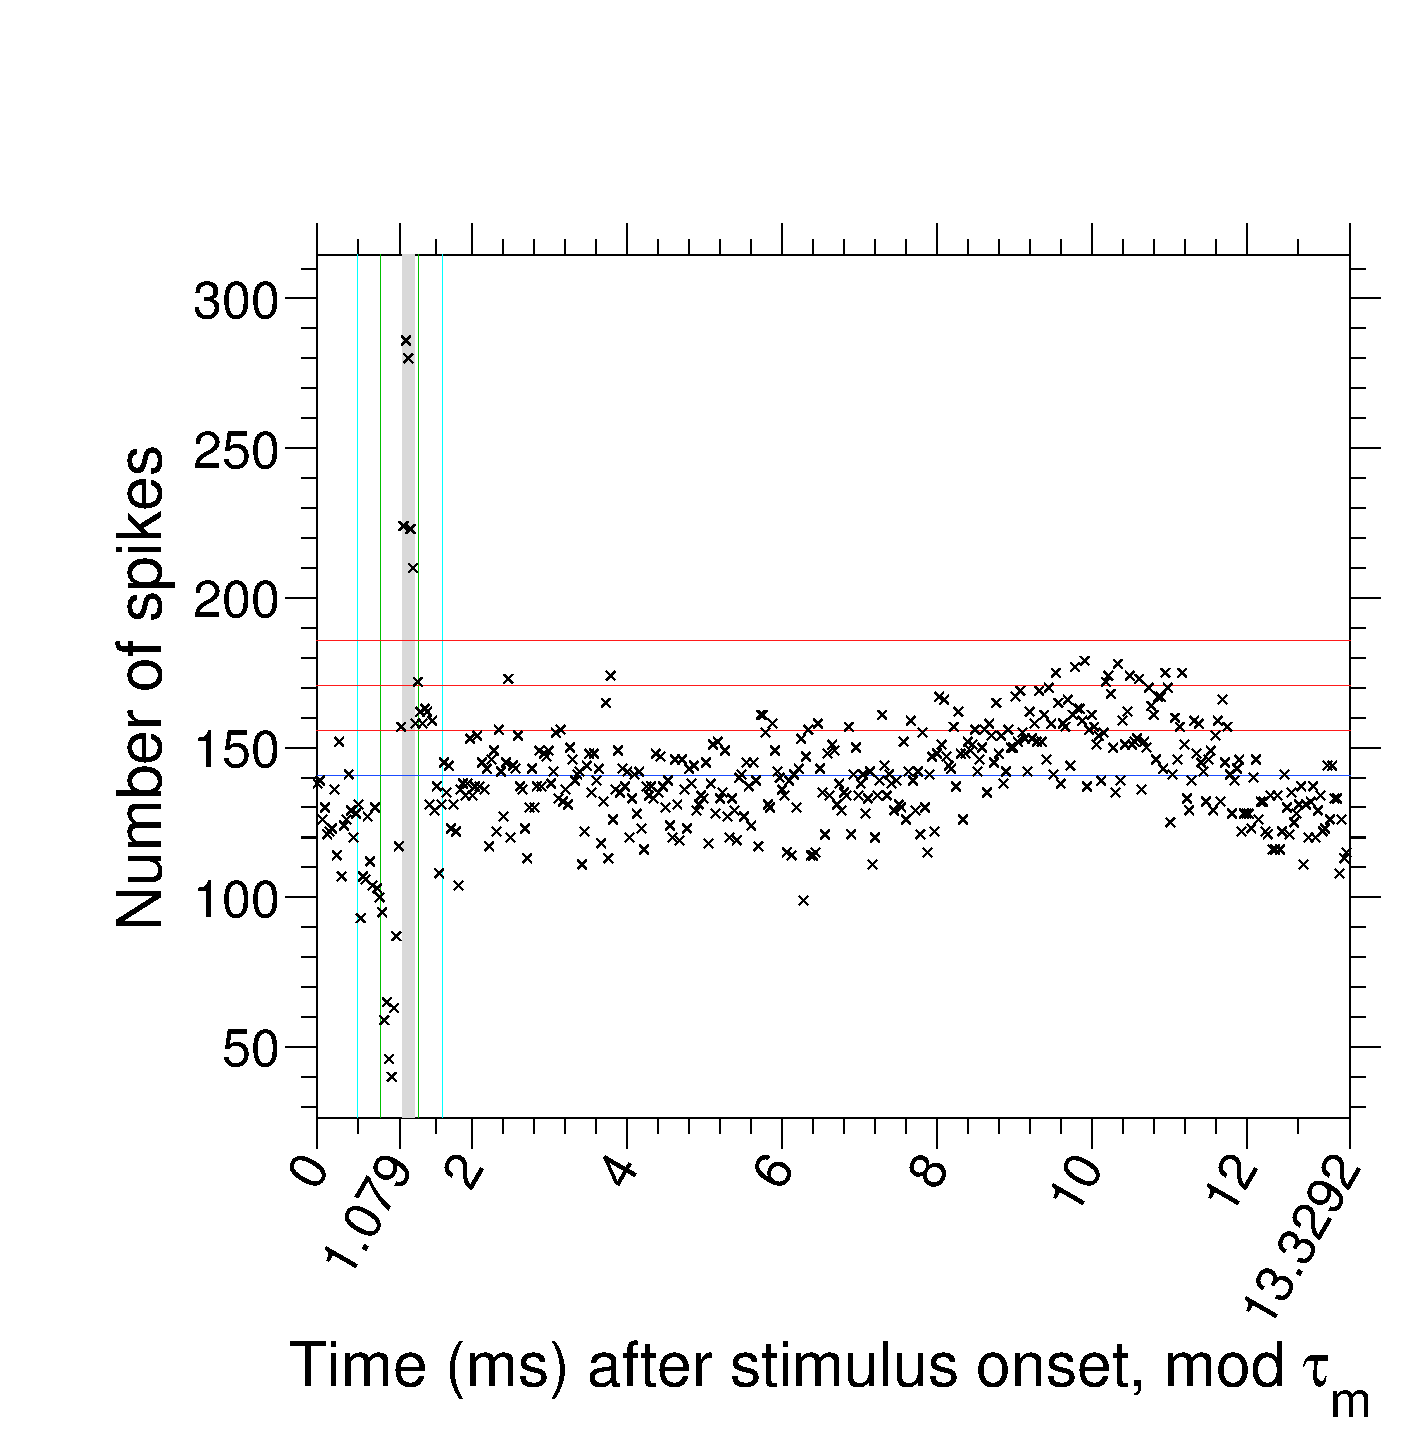
\includegraphics[width=\linewidth]{%
%%figs/info/monitor_hist_jack_v1_ch9_s56_20120817T084855.eps}
%%    \end{subfigure}
%%    \caption{Crosses: Histogram of spikes in bins of width \SI{0.030716}{ms}.
%%\ref{fig:mahist-b4}: \ac{M1} \ac{V4}, channel 4, session 336; a channel and session very strongly exhibiting the monitor artifact.
%%\ref{fig:mahist-j4}: \ac{M2} \ac{V4}, channel 41, session 31; a dataset where the artifact is not present.
%%\ref{fig:mahist-j1s51}: \ac{M2} \ac{V1}, channel 9, session 51; data strongly presenting the monitor artifact.
%%\ref{fig:mahist-j1s56}: \ac{M2} \ac{V1}, channel 9, session 56; data mildly showing the effect of the monitor artifact.
%%Green vertical lines: extremities of search window (contained between the lines).
%%Cyan vertical lines: extremities of mean region.
%%Blue line: mean of the data (excluding area between cyan lines).
%%Red lines: mean plus 1, 2 and 3 standard deviations respectively.
%%Gray background: Spikes marked as contaminated and scheduled for redaction.
%%}
%%    \label{fig:mahist}
%%\end{figure}

% INSERT HIST FIGURE 

As shown in Fig.~\ref{fig:mahist}, the analysis conforms to our expectations.
However, doing the analysis in this more rigorous manner revealed the contamination was more widespread than previously assumed.
The histograms of spike times indicate that more sessions are contaminated than not, and only a couple of channels are completely clean for every session.

For the most part, the timing of the monitor artifact $\bmod \tau_m$ is very reliable and it affects the same 6 or so bins whenever the data is contaminated.
The contaminated part of each monitor cycle is thus restricted to at most \SI{0.2}{ms}, and, assuming this period of time contains both genuine spikes and artificial spikes, if we simply delete all data points with this \SI{0.2}{ms} window, we will lose at most less than \SI{2}{\percent} of the genuine spikes.
This level of data loss is not terribly significant, and justifiable for the gain in reliability of the remaining dataset, particularly for sessions where artificial spikes seem to be more common than genuine ones.

\begin{table}[hbtp]
\caption{Typical time of the peak in number of spikes due to the monitor artifact effect.
The time is given relative to the start of the monitor refresh as given by the stimulus onset times.
Monitor artifacts occur at $t = t^*_m + k \tau_m$, for $k \in \Z$.
For channels recording from \ac{M2} \ac{V1}, the artifact will occur at one of the two stated times throughout a given session, but which of the two varies from channel-to-channel for any individual session, and from session-to-session for any individual channel.
Why this happens is unclear.}
\label{tab:mapeak}
\begin{center}
\begin{tabular}{rlc}
\toprule
Animal  & Region & Time of artifact peak $t^*_m$ $\pm 0.01$ (\si{\milli\second})
\\
\midrule
M1  & V1    & 0.95
\\
        & V4    & 0.97
\\
M2    & V1    & either 0.97 or 1.19
\\
        & V4    & 1.15
\\
\bottomrule
\end{tabular}
\end{center}
\end{table}

% However it is apparent that this method is not great (see jack v1 ch7 s57)

However, it is possible to do better that this and to isolate and remove only the contaminated bins.
As shown in Fig.~\ref{fig:mahist}, the effect of the artifact is greater for some sessions than others and
From observations on the typical width time of the width and peak time (Table.~\ref{tab:mapeak}) of the artifact, along with its periodicity ($\tau_m$), the following method of removal was devised and implemented.
\begin{enumerate}
\item Perform the modulo $\tau_m$ and take the histogram as described above.
\item Define the ``search region'' as bins which contain spike within $t^*_m \pm \SI{0.130}{ms}$, so we have one bin more than the anticipated artifact width in either direction.
      (For \ac{M2} \ac{V1}, we use the range (0.968 - 0.130 , 1.190 + 0.130)\si{\milli\second}.)
\item Find the mean, $\mu$, and standard deviation, $\sigma$, of all the bins which are at least 10 away (\SI{0.3}{ms} away) from the search region.
      We also exclude the final bin since $0.030716 \bmod \tau_m \neq 0$ and it is only part-full.
\item If any one of the bins in the search region exceeds $\mu + 3 \sigma$, we declare the session contaminated and proceed with the following steps.
      If not, it is declared intact and left as it is.
\item All bins in the search region which contain more than $\mu + 3 \sigma$ spikes are declared contaminated.
\item Let $t_m$ denote the time of the centre of the bin in the search region containing the most spikes.
\item All bins which contain spikes within $t_m \pm \SI{0.1}{ms}$ are placed in ``quarantine''.
\item All quarantined bins which contain more than $\mu + 2.5 \sigma$ spikes are declared contaminated.
\item All bins between the first and last contaminated bins are declared contaminated.
\item Consider immediate neighbours of the first bin and if they are also contain more than $\mu + 2.5 \sigma$ spikes, they are declared contaminated.
\item Repeat the above step until either a neighbour is found which is not contaminated, or until a maximum of three bins have been added to the contaminated region.
\item Consider immediate neighbours of the last bin and if they are also contain more than $\mu + 2.5 \sigma$ spikes, they are declared contaminated.
\item Repeat the above step until either a neighbour is found which is not contaminated, or until a maximum of three bins have been added to the contaminated region.
\item Consider the full dataset of spikes for this particular channel and session.
\item For each spike, consider which bin its spike time would be arranged into.
\item If it is a contaminated bin, the spike is removed from the dataset.
\end{enumerate}

This allows us to have prior assumptions about the location and width of the monitor artifact effect, but be flexible about exactly where it falls and which sets of bins are affected.
It is possible that the dynamically targeted removal method may cause issues due to inconsistency in the data across different sessions, but there is a clearly a gain in the amount of preserved data and a gain in the reliability of the data which remains.


%==============================================================================
\subsection{Misc}
%------------------------------------------------------------------------------

Neurolynx NSE files were loaded into MATLAB using the Neurolynx supplied code when operating on Windows, and an version 6 of an unofficial port for Linux (recommended by Neurolynx) otherwise.%
\footnote{Available at
\\ \url{http://www.urut.ch/new/serendipity/index.php?/pages/downloads.html}}
